\newpage
\chapter{Case Study Description}
To this day, hydrogen trucks are starting to become a reality. 
What is proposed on the market or still under development offer values of chassis occupation comparable with the ones of diesel-powered solutions.
Also, the range of such solutions is in line with what is offered today in the fossil-fueled market: $H_2$ tanks ranging from $30$ to $100$ kg can offer a range of more than $400$ km\textsuperscript{\cite{pianoidrogeno}}.

A lot of effort in the development of hydrogen powered trucks is being currently spent by joint-ventures between industries and logistic partners, like the partnership between Scania and the food wholesaler Asko; given this fact, our case study will deal with the analysis of the truck fleet needed by a sample logistic depot.

The model of truck considered is based on the\textbf{ Scania G-series} platform, produced by the aforementioned joint venture between the two Swedish companies; the vehicle has the characteristics showed in Table \ref{tab:truckdata}. We computed the size of an hypothetical hydrogen truck with an equivalent range with respect to the one powered with diesel engine.

\begin{table}[H]
\centering
\begin{tabular}{|lc|}
\hline
\multicolumn{2}{|c|}{\cellcolor{bluepoli!40}{\textbf{Scania G-series (Asko)}}}  \\ \hline
\multicolumn{1}{|l|}{Size {[}tons{]}}          & $27,00$                        \\ \hline
\multicolumn{1}{|l|}{Number of trucks}         & $10,00$                        \\ \hline
\multicolumn{1}{|l|}{Range {[}km/day{]}}       & $500,00$                       \\ \hline
\multicolumn{1}{|l|}{Motor power {[}kW{]}}     & $390,00$                       \\ \hline
\multicolumn{1}{|l|}{Battery {[}kWh{]}}        & $56,00$                        \\ \hline
\multicolumn{1}{|l|}{FC power {[}kW{]}}        & $90,00$                        \\ \hline
\multicolumn{1}{|l|}{$H_2$ tank size {[}kg{]}} & $33,00$                        \\ \hline
\end{tabular}
\caption{\textit{Truck data\textsuperscript{\cite{pianoidrogeno}}}}
\label{tab:truckdata}
\end{table}

Our case studies will focus on an Amazon Logistics depot in Milano (Via V. Toffetti, 108). Being a pretty small depot, we imagined it to be served by $10$ trucks each day, with the required amount of hydrogen showed in Table \ref{tab:hydrogenrequirements} (note that the $H_2$ provision has been considered bigger of $10\%$).

\begin{table}[H]
\centering
\begin{tabular}{|lc|}
\hline
\multicolumn{2}{|c|}{\cellcolor{bluepoli!40}{\textbf{Hydrogen Requirements}}} \\ \hline
\multicolumn{1}{|l|}{$H_2$ daily needs {[}kg/day{]}}     & $363,00$           \\ \hline
\multicolumn{1}{|l|}{LHV $H_2$ {[}kWh/kg{]}}             & $33,31$            \\ \hline
\multicolumn{1}{|l|}{LHV $H_2$ {[}MJ/kg{]}}              & $119,92$           \\ \hline
\multicolumn{1}{|l|}{Electric energy required {[}MWh{]}} & $20,46$            \\ \hline
\end{tabular}
\caption{Hydrogen requirements}
\label{tab:hydrogenrequirements}
\end{table}

The provision of hydrogen to serve the daily needs of the depot has been considered analysing different solutions. The focus is put on an \textbf{electrolysis system}, with the energy produced from \textbf{hydroelectric} and \textbf{photovoltaic} plants. In Figure \ref{fig:electrolyser} we can see the chosen PEM electrolyser, whose characteristics can be seen in Table \ref{tab:specshydrolyser}.

\begin{figure}[H]
\centering
    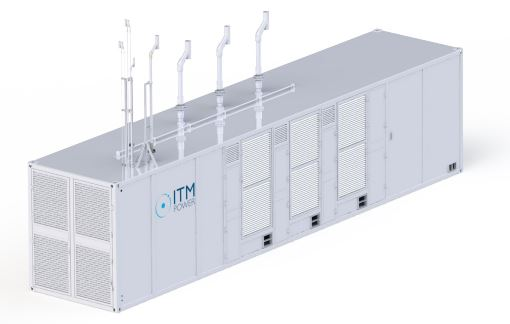
\includegraphics[width=0.5\textwidth]{Chapters/Pictures/HGas 3SP.JPG}
    \caption{Hgas3SP electrolyser by \textbf{ITM power}\textsuperscript{\cite{HGas3SP}}}
    \label{fig:electrolyser}
\end{figure}

\begin{table}[h]
\centering
\begin{tabular}{|l|l|}
\hline
\rowcolor{bluepoli!40}             
\multicolumn{2}{|c|}{\textbf{Tech Specs}}                                                                       \\ \hline
\multicolumn{1}{|l|}{Ectrolyser technology}                   & \multicolumn{1}{c|}{PEM}                        \\ \hline
\multicolumn{1}{|l|}{Number of stacks}                        & \multicolumn{1}{c|}{3}                          \\ \hline
\multicolumn{1}{|l|}{System packaging and size}               & \multicolumn{1}{c|}{1 x 20 ft \& 1 x 40 ft ISO} \\ \hline
\multicolumn{1}{|l|}{Power supply}                            & \multicolumn{1}{c|}{11kV AC (3 Phase - $50Hz$)} \\ \hline
\multicolumn{1}{|l|}{Control}                                 & \multicolumn{1}{c|}{PLC}                        \\ \hline
\multicolumn{1}{|l|}{Hydrogen generation pressure [bar]}      & \multicolumn{1}{c|}{20}                         \\ \hline
\multicolumn{1}{|l|}{Hydrogen purity (ISO standard)}          & \multicolumn{1}{c|}{Up to $99,999\%$}           \\ \hline
\multicolumn{1}{|l|}{Maximum hydrogen production appx [kg/h]} & \multicolumn{1}{c|}{$36,00$}                    \\ \hline
\multicolumn{1}{|l|}{Input power at maximum appx [kW]}        & \multicolumn{1}{c|}{$2.350,00$}                 \\ \hline
\end{tabular}
\caption{\textit{Technical specifications of HGas3SP}}
\label{tab:specshydrolyser}
\end{table}

\newpage
\section{Hydroelectric Power}
\subsection{Electrolyser in the Depot}

This first solution is based on these assumptions:

\begin{description}
    \item[\textbf{Electricity Production}] It is produced by the Hydroelectric PP in \textbf{Crodo} (VB) (see Table \ref{tab:crodotechspec}) and then is transferred to Milano via the electric grid;
    \item[\textbf{Electrolysis}] It is performed on site in the depot, with a system\textbf{ owned by the logistics company}.
\end{description}

\begin{table}[h]
\centering
\begin{tabular}{|lc|}
\hline
\rowcolor{bluepoli!40}\multicolumn{2}{|c|}{\textbf{Hydropower Plant - Crodo}}      \\ \hline
\multicolumn{1}{|l|}{Efficient power {[}kW{]}}                      & $52.800,00$  \\ \hline
\multicolumn{1}{|l|}{Distance from depot {[}km{]}}                  & $160,00$     \\ \hline
\multicolumn{1}{|l|}{V$_{Line}$ {[}V{]}}                            & $200.000,00$ \\ \hline
\multicolumn{1}{|l|}{I$_{Line}$ {[}A{]}}                            & $264,00$     \\ \hline
\multicolumn{1}{|l|}{Power loss {[}\%{]} (HV systems)}              & $0,02$       \\ \hline
\multicolumn{1}{|l|}{Effective power {[}kW{]}}                      & $51.744,00$  \\ \hline
\end{tabular}
\caption{\textit{Techinical data of \href{https://goo.gl/maps/dqKiAsYcyXrGMbUd6}{Crodo's Hydropower Plant}}}
\label{tab:crodotechspec}
\end{table}

\subsection{External Electrolyser, Transport of Hydrogen}
The second solution is based on these assumptions:

\begin{description}
    \item[\textbf{Electricity Production}] It is produced by the Hydroelectric PP in \textbf{Trezzo sull'Adda} (MI) (see Table \ref{tab:trezzoaddaspec});
    \item[\textbf{Electrolysis}] It is performed on site \textbf{in the Hydroelectric PP}; the system is \textbf{not owned by the logistics company}.
\end{description}

\begin{table}[hb!]
\centering
\begin{tabular}{|lc|}
\hline
\rowcolor{bluepoli!40}\multicolumn{2}{|c|}{\textbf{Hydroelectric Power plant - Trezzo Sull'Adda}} \\ \hline
\multicolumn{1}{|l|}{Efficient power {[}kW{]}}              & $10.500,00$                         \\ \hline
\multicolumn{1}{|l|}{Mean producible energy {[}kWh{]}}      & $65.000.000,00$                     \\ \hline
\multicolumn{1}{|l|}{Distance from depot {[}km{]}}          & $40,00$                             \\ \hline
\multicolumn{1}{|l|}{$V_{Line}$ {[}V{]}}                    & $200.000,00$                        \\ \hline
\multicolumn{1}{|l|}{$Current_{Line}$ {[}A{]}}              & $52,50$                             \\ \hline
\multicolumn{1}{|l|}{Power loss [\%] (HV systems)}          & $0,02$                              \\ \hline
\multicolumn{1}{|l|}{Effective power {[}kW{]}}              & $10.290,00$                         \\ \hline
\end{tabular}
\caption{Techinical data of \href{https://g.page/centrale-idroelettrica-taccani?share}{Trezzo sull'Adda Hydropower plant}}
\label{tab:trezzoaddaspec}
\end{table}

\newpage
The hydrogen is directly bought from the owner of the electrolyser, and is then delivered to the depot in Milano using diesel powered \textbf{Euro VI trucks}. The main characteristics of this power plant are reported in the table below. This hydroelectric power plant is different from the one considered in the first solution: in fact, it uses the flow of river \textbf{Adda} instead of the potential energy. The choice of this power plant was driven by its short distance from Milano, that could make transport of $H_2$ faster and more efficient.

\section{Photovoltaic Power}

\subsection{PV Plant in Puglia, Transport of Hydrogen}
In this case, we decided to place the hydrogen production in the  already present solar park near \textbf{Troia (FG)} in \textbf{Puglia}. This solution allowed us to collect a greater amount of solar energy, thanks to a warmer and sunnier climate and a more favourable angle of incidence (the nearer to the equator, the better). The hydrogen is produced on site, so the problem would be to move it to the depot in \textbf{Milano}, with a consequent increase in \textbf{transportation costs} and \textbf{$CO_2$ emissions}. In Table \ref{tab:costconstant} are showed some important cost values, while in Table \ref{tab:pvbessass} are shown the assumptions made about the efficiency of the system.

\begin{table}[hb!]
\centering
\begin{tabular}{|lc|}
\hline
\rowcolor{bluepoli!40}\multicolumn{2}{|c|}{\textbf{Constant}}                             \\ \hline
\multicolumn{1}{|l|}{Electricity cost {[}€/kWh{]}}              & 0,22                    \\ \hline
\multicolumn{1}{|l|}{Electricity Selling revenue {[}€/kWh{]}}   & 0,10                    \\ \hline
\multicolumn{1}{|l|}{Cost of battery {[}€/kWh{]}}               & 122,13                  \\ \hline
\multicolumn{1}{|l|}{Hydrogen transportation cost {[}€/kg{]}}   & 3,00                    \\ \hline
\multicolumn{1}{|l|}{Cost of a solar panel {[}€{]}}         & 811,88                \\ \hline
\multicolumn{1}{|l|}{Hydrogen storage cost {[}€/kg{]}}          & 0,04                    \\ \hline
\multicolumn{1}{|l|}{Compression {[}kWh$_el$/kWh$_{H_2}${]}}    & 0,10                    \\ \hline
\end{tabular}
\caption{\textit{Useful cost constant\textsuperscript{\cite{ARERA2020,enelx, pianoidrogeno}}}}
\label{tab:costconstant}
\end{table}

\begin{table}[h!]
\centering
\begin{tabular}{|lc|}
\hline
\rowcolor{bluepoli!40}\multicolumn{2}{|c|}{\textbf{Efficiency assumptions}}                 \\ \hline
\multicolumn{1}{|l|}{BESS Charging efficiency}   & \textbf{$0,95$}                          \\ \hline
\multicolumn{1}{|l|}{BESS Self discharge}        & \textbf{$0,90$}                          \\ \hline
\multicolumn{1}{|l|}{BESS discharge}             & \textbf{$0,97$}                          \\ \hline
\multicolumn{1}{|l|}{Plant efficiency}           & \textbf{$0,80$}                          \\ \hline
\multicolumn{1}{|l|}{RTE efficiency}             & \textbf{$0,83$}                          \\ \hline
\multicolumn{1}{|l|}{Energy required {[}MWh{]}}  & \textbf{$23,72$}                         \\ \hline
\end{tabular}
\caption{Phototovoltaic and BESS efficiency assumptions}
\label{tab:pvbessass}
\end{table}

\newpage
In Table \ref{tab:hpuglia} is possible to see the irradiation coefficients of the chosen plant.

\begin{table}[h!]
\centering
\begin{tabular}{|l|l|c|}
\hline
\rowcolor{bluepoli!40} \textbf{Month} & \textbf{Days} & $\textbf{H }[kWh/m^2\cdot month]$ \\ \hline
1              & 31            & $105,68$       \\ \hline
2              & 28            & $108,01$       \\ \hline
3              & 31            & $125,45$       \\ \hline
4              & 30            & $176,99$       \\ \hline
5              & 31            & $193,44$       \\ \hline
6              & 30            & $187,80$       \\ \hline
7              & 31            & $215,53$       \\ \hline
8              & 31            & $204,94$       \\ \hline
9              & 30            & $165,46$       \\ \hline
10             & 31            & $135,13$       \\ \hline
11             & 30            & $121,34$       \\ \hline
12             & 31            & $112,82$       \\ \hline
\end{tabular}
\caption{\textit{Irradiation coefficient per month in Puglia\textsuperscript{\cite{PVINFOSYSTEM}}}}
\label{tab:hpuglia}
\end{table}

\subsection{PV Plant in Milano, Electrolyser in the Depot}
In this other case study the PV plant is built on the roof of the depot in Milano: the situation will be reversed with respect to the previous one, having in northern Italy a lower irradiation coefficient (see Table \ref{tab:hmilan}). This will penalize the solution from the point of view of the collected solar energy, but at the same time it will have lower transportation costs, because the PV plant, the electrolyser and the depot are all in the same site.

\begin{table}[p]
\centering
\begin{tabular}{|l|l|c|}
\hline
\rowcolor{bluepoli!40} \textbf{Month} & \textbf{Days} & \multicolumn{1}{l|}{\textbf{H}$[kWh/m^2\cdot month]$} \\ \hline
1              & 31            & $20,6$                          \\ \hline
2              & 28            & $33,9$                          \\ \hline
3              & 31            & $57,4$                          \\ \hline
4              & 30            & $90,9$                          \\ \hline
5              & 31            & $136,5$                         \\ \hline
6              & 30            & $145,2$                         \\ \hline
7              & 31            & $184,8$                         \\ \hline
8              & 31            & $184,4$                         \\ \hline
9              & 30            & $147,9$                         \\ \hline
10             & 31            & $85,4$                          \\ \hline
11             & 30            & $32,1$                          \\ \hline
12             & 31            & $22,5$                          \\ \hline
\end{tabular}
\caption{Irradiation coefficient per month in Milan}
\label{tab:hmilan}
\end{table}

In both cases we will face out with the problem of storing energy as electricity (with a BESS) or as hydrogen, producing more hydrogen of the necessary, to eventually sell it.